%%%%%%%%%%%%%%%%%%%%%%%%%%%%%%%%%%%%%%%%%
% University/School Laboratory Report
% LaTeX Template
% Version 3.1 (25/3/14)
%
% This template has been downloaded from:
% http://www.LaTeXTemplates.com
%
% Original author:
% Linux and Unix Users Group at Virginia Tech Wiki 
% (https://vtluug.org/wiki/Example_LaTeX_chem_lab_report)
%
% License:
% CC BY-NC-SA 3.0 (http://creativecommons.org/licenses/by-nc-sa/3.0/)
%
%%%%%%%%%%%%%%%%%%%%%%%%%%%%%%%%%%%%%%%%%

%----------------------------------------------------------------------------------------
%	PACKAGES AND DOCUMENT CONFIGURATIONS
%----------------------------------------------------------------------------------------

\documentclass{article}

\usepackage{polski}
\usepackage{array}
\usepackage[utf8]{inputenc}
\usepackage{booktabs}
\usepackage{multirow}
\usepackage{caption}

\usepackage[version=3]{mhchem} % Package for chemical equation typesetting
\usepackage{siunitx} % Provides the \SI{}{} and \si{} command for typesetting SI units
\usepackage{graphicx} % Required for the inclusion of images
\usepackage{natbib} % Required to change bibliography style to APA
\usepackage{amsmath} % Required for some math elements 

\setlength\parindent{0pt} % Removes all indentation from paragraphs

\renewcommand{\labelenumi}{\alph{enumi}.} % Make numbering in the enumerate environment by letter rather than number (e.g. section 6)
\newcommand{\rowstyle}[1]{\gdef\currentrowstyle{#1}%
  #1\ignorespaces
}
%\usepackage{times} % Uncomment to use the Times New Roman font

%----------------------------------------------------------------------------------------
%	DOCUMENT INFORMATION
%----------------------------------------------------------------------------------------

\title{Ćwiczenie nr 82: Efekt fotoelektryczny} % Title

\author{Rafał \textsc{Grabiański} i Zbigniew \textsc{Królikowski}} % Author name

\date{\today} % Date for the report

\addtolength{\oddsidemargin}{-.875in}
\addtolength{\evensidemargin}{-.875in}
\addtolength{\textwidth}{1.75in}
\addtolength{\topmargin}{-.875in}
\addtolength{\textheight}{1.75in}

\begin{document}

% Please add the following required packages to your document preamble:
% \usepackage{booktabs}
\begin{table}[h]
\begin{tabular}{@{}llllll@{}}
\toprule
\begin{tabular}[c]{@{}l@{}}Wydział:\\ \\ WIEiT\end{tabular}                                    & \multicolumn{2}{l}{\begin{tabular}[c]{@{}l@{}}Imię i nazwisko:\\ Rafał Grabiański\\ Zbigniew Królikowski\end{tabular}}                & \begin{tabular}[c]{@{}l@{}}Rok:\\ \\ II\end{tabular}            & \begin{tabular}[c]{@{}l@{}}Grupa:\\ \\ 7\end{tabular}              & \begin{tabular}[c]{@{}l@{}}Zespół:\\ \\ 7\end{tabular} \\ \midrule
\multicolumn{1}{|c|}{\begin{tabular}[c]{@{}c@{}}PRACOWNIA\\ FIZYCZNA\\ WFiIS AGH\end{tabular}} & \multicolumn{4}{l|}{Temat: Modelowanie pola}                                                                                                                                                                                                                                                  & \multicolumn{1}{l|}{Nr ćwiczenia: 31}                     \\ \midrule
\begin{tabular}[c]{@{}l@{}}Data wykonania:\\ \\ \\ 28.10.2014\end{tabular}                     & \begin{tabular}[c]{@{}l@{}}Data oddania: \\ \\ \\ 4.11.2014\end{tabular} & \begin{tabular}[c]{@{}l@{}}Zwrot do poprawy:\\ \\ \\ 25.11.2014\end{tabular} & \begin{tabular}[c]{@{}l@{}}Data oddania: \\ \\ \\ 2.12.2014\end{tabular} & \begin{tabular}[c]{@{}l@{}}Data zaliczenia:\\ \\ \\ .\end{tabular} & OCENA:                                                  \\ \bottomrule
\end{tabular}
\end{table}

%\maketitle % Insert the title, author and date

% If you wish to include an abstract, uncomment the lines below


%----------------------------------------------------------------------------------------
%	SECTION 1 - CEL ĆWICZENIA
%----------------------------------------------------------------------------------------

\section{Cel ćwiczenia}
Celem ćwiczenia było poznanie podstawowych wielkości opisujących pole elektryczne poprzez wyznaczenie linii ekwipotencjalnych i wektorów natężenia pola elektrycznego na płaszczyźnie dla różnych konfiguracji elektrod.


% If you have more than one objective, uncomment the below:
%\begin{description}
%\item[First Objective] \hfill \\
%Objective 1 text
%\item[Second Objective] \hfill \\
%Objective 2 text
%\end{description}



%\clearpage

%----------------------------------------------------------------------------------------
%	SECTION 2
%----------------------------------------------------------------------------------------
\section{Wyniki pomiarów}
\subsection{Wariant A - kondensator płaski}
\begin{table}[htbp]
\centering
\scalebox{0.9}{
\begin{tabular}{|c|c|c|c|c|c|c|c|c|}
\hline
L.p. & \multicolumn{ 1}{c|}{x [mm]} &\multicolumn{ 1}{c|}{$V_{a} [V]$} &\multicolumn{ 1}{c|}{$V_{b} [V]$} & \multicolumn{ 1}{c|}{$V_{c} [V]$}& \multicolumn{ 1}{c|}{$V_{dośw}$} & \multicolumn{1}{c|}{$V_{teor}$} & \multicolumn{1}{c|}{$V_{d}$ [V]} & \multicolumn{1}{c|}{Ve [V]} \\ \cline{ 1- 1}\cline{ 2- 9}
0 & 0 & 0 & 0 & 0 & 0 & \multicolumn{1}{c|}{0} & 0 & 0 \\ \hline
1 & 6 & 1.26 & 1.26 & 1.21 & 1.2433333333 & 1.18 & 1.77 & 1.57 \\ \hline
2 & 11 & 2.15 & 2.18 & 2.09 & 2.14 & 2.16 & 2.84 & 2.19 \\ \hline
3 & 16 & 3.19 & 3.36 & 2.99 & 3.18 & 3.14 & 3.7 & 3.15 \\ \hline
4 & 21 & 4.19 & 4.2 & 3.87 & 4.0866666667 & 4.12 & 4.24 & 4.24 \\ \hline
5 & 26 & 5.02 & 5.04 & 4.99 & 5.0166666667 & 5.10 & 5.08 & 5.1 \\ \hline
6 & 31 & 5.87 & 5.98 & 5.99 & 5.9466666667 & 6.08 & 5.32 & 5.59 \\ \hline
7 & 36 & 6.99 & 7.02 & 6.9 & 6.97 & 7.06 & 6.73 & 7.05 \\ \hline
8 & 41 & 7.93 & 7.94 & 7.74 & 7.87 & 8.04 & 7.65 & 7.93 \\ \hline
9 & 46 & 8.91 & 9.01 & 8.76 & 8.8933333333 & 9.02 & 8.51 & 8.93 \\ \hline
10 & 51 & 10 & 10 & 10 & 10 & \multicolumn{1}{c|}{10} & 10 & 10 \\ \hline
\end{tabular}
}
\caption{Wyniki pomiarów i obliczeń dla płaskiego układu elektrod}
\label{tab:ch01}
\end{table}

\begin{table}[h!tbp]
\centering
\scalebox{0.8}{
\begin{tabular}{|c|c|c|c|}
\hline
L.p. & x [mm] & $E_{dośw} [\frac{V}{m}]$ & $E_{teor} [\frac{V}{m}]$  \\ \cline{ 1-4}
0 & 3 & 207.2222222222 & 196.08 \\ \hline
1 & 8.5 & 179.3333333333 & 196.08 \\ \hline
2 & 13.5 & 208 & 196.08 \\ \hline
3 & 18.5 & 181.3333333333 & 196.08 \\ \hline
4 & 23.5 & 186 & 196.08 \\ \hline
5 & 28.5 & 186 & 196.08 \\ \hline
6 & 33.5 & 204.6666666667 & 196.08 \\ \hline
7 & 38.5 & 180 & 196.08 \\ \hline
8 & 43.5 & 204.6666666667 & 196.08 \\ \hline
9 & 48.5 & 221.3333333333 & 196.08 \\ \hline
\end{tabular}
}
\caption{Obliczone natężenie pola z danych doświadczalnych i teoretycznych}
\label{}
\end{table}

\clearpage
\begin{figure}{l}
	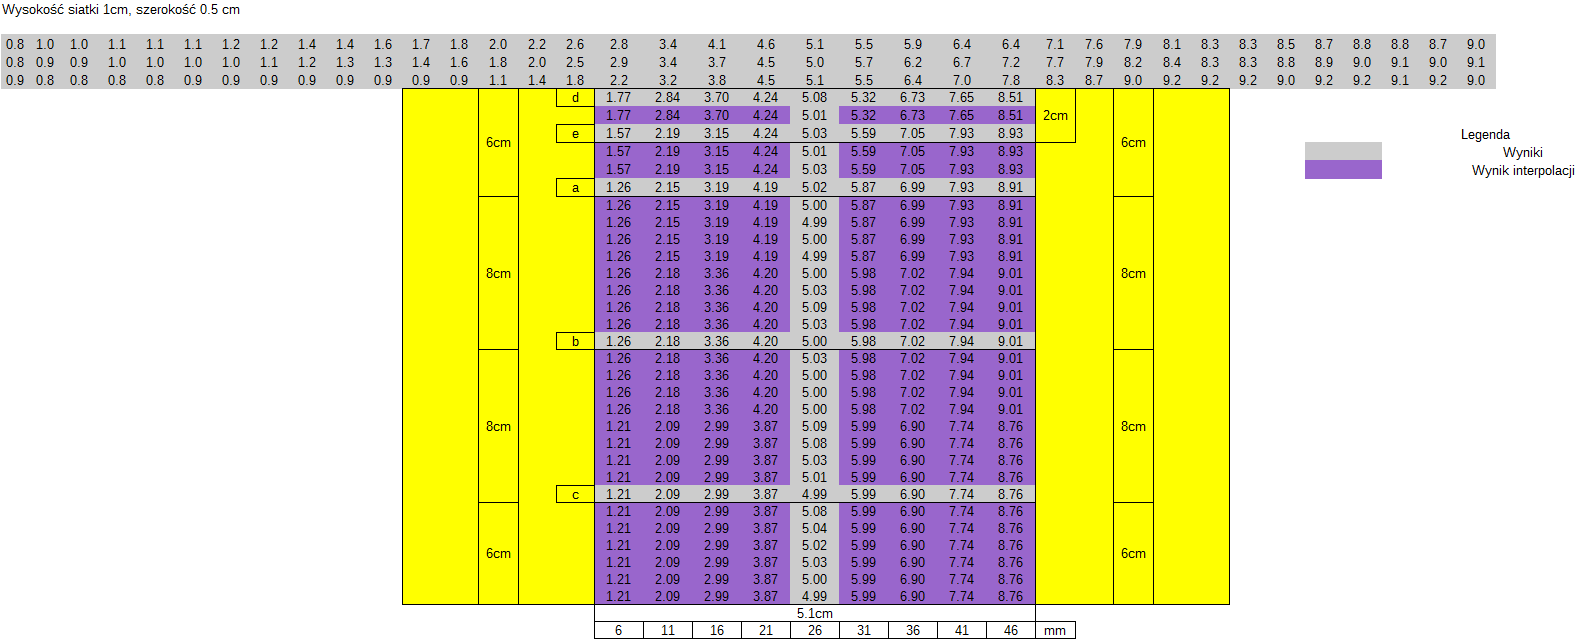
\includegraphics[scale=0.43]{pic1}
	\caption{Wyniki zmierzonego potencjału dla kondensatora płaskiego naniesione na rysunek}
\end{figure}

\subsection{Wariant B - kondensator cylindryczny}

\begin{table}[htbp]
\centering
\scalebox{0.9}{
\begin{tabular}{|c|c|c|c|c|c|c|}
\hline
L.p. & x [mm] & $V_{a} [V]$ & $V_{b} [V]$ & $V_{c} [V]$ & $V_{dosw} [V]$ & \multicolumn{1}{c|}{V teor} \\ \hline
0 & 0 & 10 & 10 & 10 & 10 & \multicolumn{1}{c|}{0} \\ \hline
1 & 7 & 7.82 & 8.03 & 8.05 & 7.9666666667 &  8.09\\ \hline
2 & 15 & 6.28 & 6.43 & 5.97 & 6.2266666667 &  6.43\\ \hline
3 & 22 & 5.13 & 5.27 & 4.76 & 5.0533333333 &  5.25\\ \hline
4 & 30 & 4.17 & 4.29 & 3.79 & 4.0833333333 &  4.12\\ \hline
5 & 37 & 3.34 & 3.47 & 2.95 & 3.2533333333 &  3.27\\ \hline
6 & 45 & 2.6 & 2.68 & 2.22 & 2.5 &  2.41\\ \hline
7 & 52 & 1.9 & 1.98 & 1.6 & 1.8266666667 & 1.75 \\ \hline
8 & 60 & 1.2 & 1.38 & 1.1 & 1.2266666667 &  1.06\\ \hline
9 & 67 & 0.68 & 0.78 & 0.56 & 0.6733333333 &  0.50\\ \hline
10 & 74 & 0 & 0 & 0 & 0 & \multicolumn{1}{c|}{10} \\ \hline
\end{tabular}
}
\caption{Wyniki pomiarów i obliczeń dla cylindrycznego układu elektrod}
\label{}
\end{table}

\begin{table}[h!tbp]
\centering
\scalebox{0.95}{
\begin{tabular}{|c|c|c|c|}
\hline
L.p. & $x [mm]$ & $E_{dośw} [\frac{V}{m}]$ & $E_{teor} [\frac{V}{m}]$  \\ \hline
0 & 3.5 & -290.4761904762 & -324.05 \\ \hline
1 & 11 & -217.5 & -248.11 \\ \hline
2 & 18.5 & -167.619047619 & -201.00 \\ \hline
3 & 26 & -121.25 & -168.92 \\ \hline
4 & 33.5 & -118.5714285714 &  -145.68  \\ \hline
5 & 41 & -94.1666666667 & -128.05 \\ \hline
6 & 48.5 & -96.1904761905 & -114.24\\ \hline
7 & 56 & -75 &  -103.11\\ \hline
8 & 63.5 & -79.0476190476 & -93.96 \\ \hline
9 & 70.5 & -96.1904761905 & -86.77 \\ \hline
\end{tabular}
}
\caption{Obliczone natężenie pola z danych doświadczalnych i teoretycznych}
\label{}
\end{table}

\clearpage

\subsection{Wariant C - dowolny układ elektrod}

\begin{figure}[h]
	\centering
	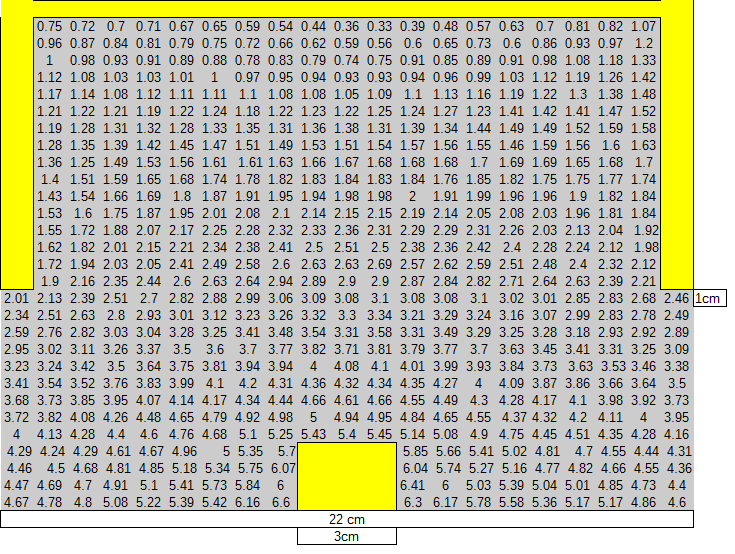
\includegraphics[scale=0.75]{pic2}
	\caption{Wyniki zmierzonego potencjału dla układu dowolnego naniesione na rysunek}
\end{figure}

%----------------------------------------------------------------------------------------
%	SECTION 5 - WYNIKI
%----------------------------------------------------------------------------------------

\section{Opracowanie wyników}

\subsection{Wariant A - kondensator płaski}
\subsubsection{Obliczenie wartości doświadczalnych natężenia pola}
Zauważamy, że nie licząc krańców kondensatora dla stałej odległości od elektrod obserwujemy stały potencjał. Uśredniamy jego wartość korzystając z trzech osi: A, B i C, licząc: $V_{dośw} = \frac{V_{a}+V_{b}+V_{c}}{3}$. Wyniki zamieściliśmy w kolumnie $V_{dośw}$ w tabeli 1.
Korzystając ze wzoru:
\begin{equation}
	E_{dośw} = \frac{V_{n+1}-V_{n}}{x_{n+1}-x_{n}}
\end{equation}
Wyliczamy wartości doświadczalne natężeń, które przypisuje punktom leżącym pomiędzy punktami pomiarowymi potencjału.
\begin{equation}
	x^{*} = \frac{x_{n+1}+x_{n}}{2}
\end{equation}
Wyniki umieściliśmy w tabeli 2.

\subsubsection{Wykresy V(x) i E(x) dla kondensatora płaskiego}
Wiedząc, że potencjał zmienia się w kondensatorze płaskim liniowo względem x:
\begin{equation}
	V(x) = \frac{U}{d} \cdot x
\end{equation}
Znając U = 10 V oraz d = 5.1 cm liczymy teoretyczne wartości potencjału wg powyższego wzoru i wpisujemy je w kolumnie $V_{dośw}$. \newline

\begin{figure}
	\centering
	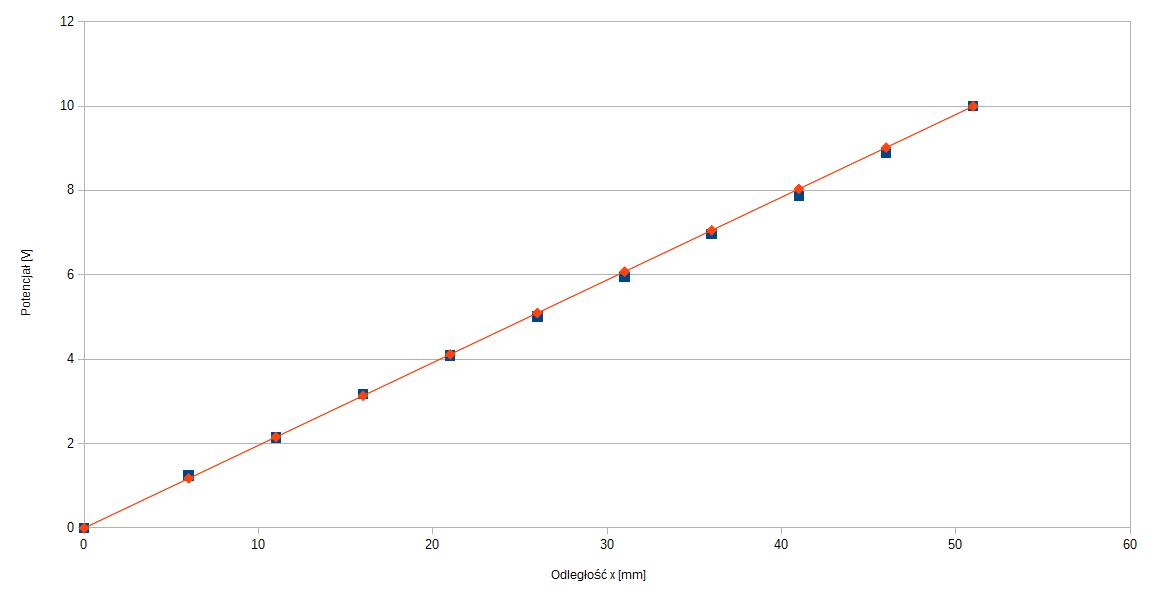
\includegraphics[scale=0.42]{ch01}
	\caption{Zależność potencjału V [V] od położenia x [mm]. Niebieskie punkty odpowiadają pomiarom doświadczalnym, pomarańczowa linia została wyprowadzona teoretycznie.}
\end{figure}

W kondensatorze płaskim natężenie pola elektrycznego pomiędzy okładkami jest stałe i dane wzorem:
\begin{equation}
	E = \frac{U}{d}
\end{equation}
Podstawiając dane mamy zatem: $E \approx 196.08 \frac{V}{m} $.
Licząc z regresji 
Poniższy wykres porównuje dane uzyskane w poprzednim podpunkcie z wartością natężenia obliczoną teoretycznie.

\begin{figure}[h!]
	\centering
	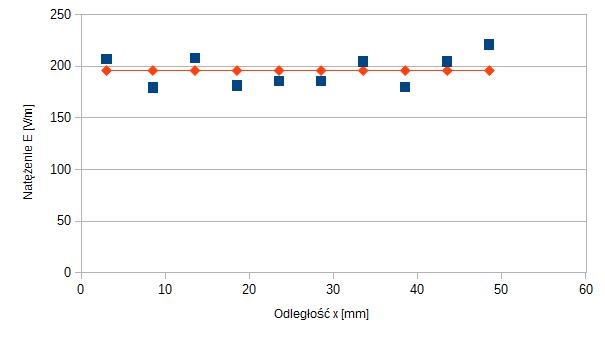
\includegraphics[scale=0.55]{ch02}
	\caption{Zależność natężenia pola E $[\frac{V}{m}]$ od położenia x [mm]. Na niebiesko punkty obliczone lokalnie na podstawie doświadczenia, pomarańczowa linia to natężenie obliczone teoretycznie.}
\end{figure}

\subsubsection{Linie ekwipotencjalne i linie pola dla kondensatora płaskiego}
Korzystając z MATLAB'a, po wprowadzeniu uzyskanych danych otrzymujemy rysunki:
\begin{figure}[h]
	\centering
	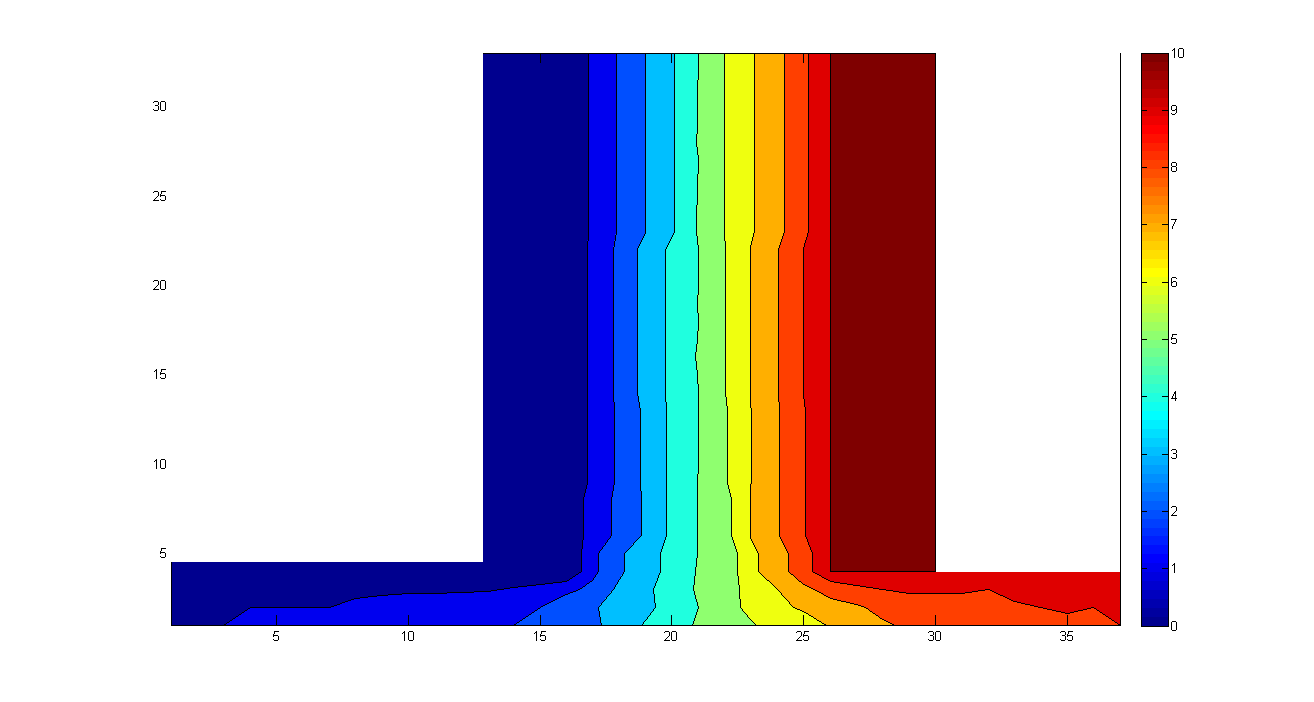
\includegraphics[scale=0.32]{plaskicontour}
	\caption{Powierzchnie ekwipotencjalne dla kondensatora płaskiego, uzyskane w rozdzielczości 1 V}
\end{figure}

\begin{figure}[h]
	\centering
	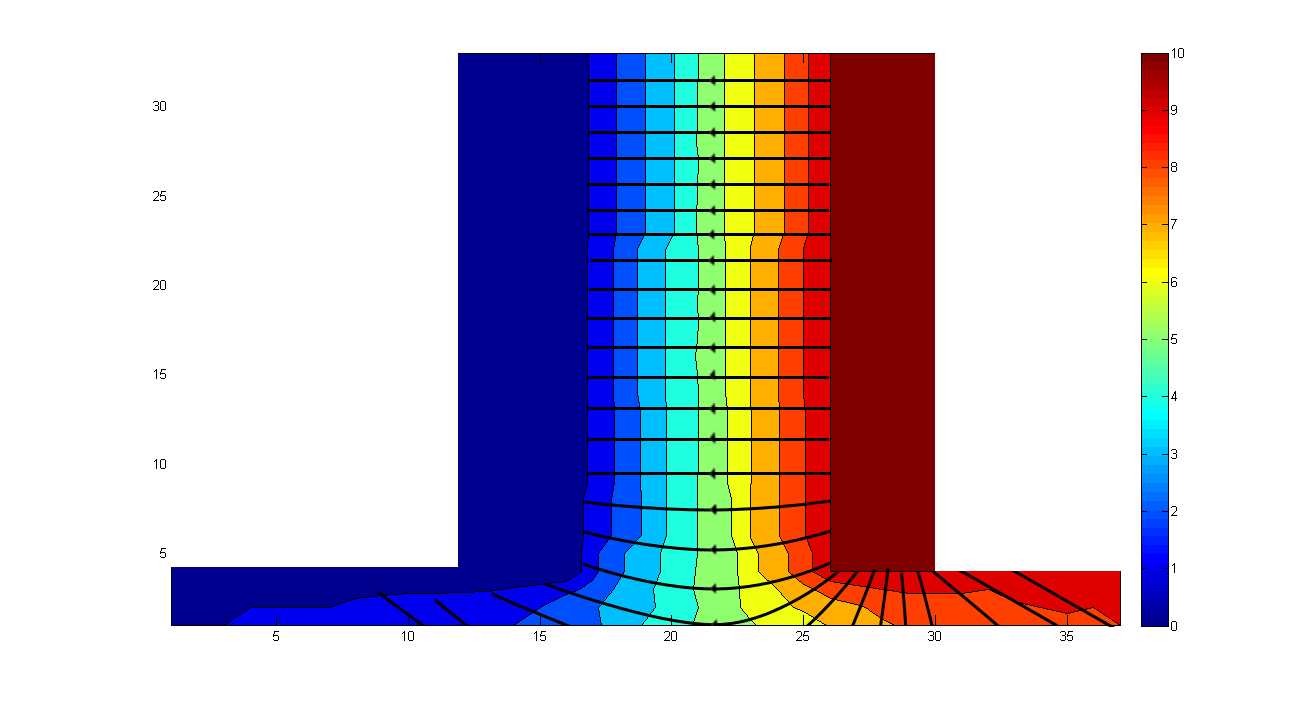
\includegraphics[scale=0.32]{plaskicontourLINIE}
	\caption{Dorysowane "ręcznie" linie natężenia pola wewnątrz i na zewnątrz kondensatora}
\end{figure}

\begin{figure}[h!]
	\centering
	\includegraphics[scale=0.45]{plaski3D}
	\caption{Powierzchnie ekwipotencjalne kondensatora płaskiego przedstawione w trójwymiarze}
\end{figure}

\begin{table}[h!tbp]
\centering
\begin{tabular}{|r|r|r|r|}
\hline
\multicolumn{1}{|l|}{Nr punktu} & \multicolumn{1}{l|}{E\_\{x\}} & \multicolumn{1}{l|}{E\_\{y\}} & \multicolumn{1}{l|}{|E|} \\ \hline
1 & 40 & -20 & 44.7 \\ \hline
2 & 100 & 60 & 116.6 \\ \hline
\end{tabular}
\label{}
\caption{Wyniki obliczenia natężenia pola w wybranych punktach}
\end{table}


\subsection{Wariant B - kondensator cylindryczny}
\subsubsection{Obliczenie wartości doświadczalnych natężenia pola}
Podobnie jak w punkcie 3.1.1, korzystając ze wzorów (1) i (2) oraz wyników pomiaru potencjału, wyliczamy natężenie pola wewnątrz kondensatora cylindrycznego dla różnych położeń. \newline Wyniki umieściliśmy w tabeli 4.
\subsubsection{Wykresy V(x) i E(x) dla kondensatora cylindrycznego}
Dany mamy wzór na potencjał w kondensatorze cylindrycznym w zależności od r:
\begin{equation}
	V(r) = \frac{U}{ln(\frac{r_{z}}{r_{w}})} \cdot ln(\frac{r}{r_{z}})
\end{equation}
Gdzie $U$ - napięcie między okładkami kondensatora, $r_{z}$ - promień zewnętrzny, $r_{w}$ - promień wewnętrzny.

Możemy więc policzyć za pomocą tego wzoru wartości teoretyczne jakie powinien uzyskiwać kondensator.
Podstawiając $r_{w} = 21 mm$ oraz $r_{z} = 95 mm$. Liczymy teoretyczne wartości potencjału. Wyniki znajdują się w tabeli 3, w kolumnie $V_{teor}$

\begin{figure}[h!]
	\centering
	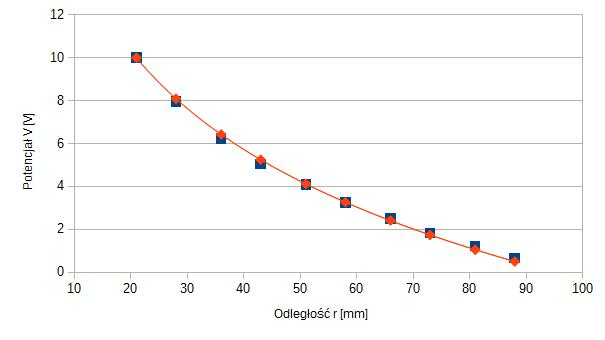
\includegraphics[scale=0.55]{ch03}
	\caption{Zależność potencjału V [V] od położenia x [mm] dla kondensatora cylindrycznego. Wartości teoretyczne odwzorowuje pomarańczowa linia, dane doświadczalne to niebieskie punkty.}
\end{figure}

Teoretyczną zależność na natężenie otrzymamy licząc pochodną cząstkową: $\frac{\partial V}{\partial r} = -\frac{U}{r \cdot ln(\frac{r_{z}}{r_{w}})}$

\begin{figure}[h!]
	\centering
	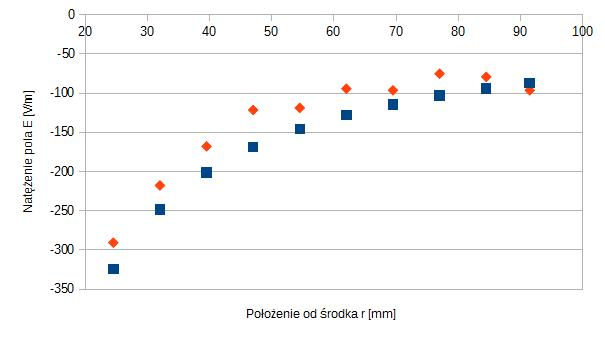
\includegraphics[scale=0.45]{ch04}
	\caption{Zależność natężenia pola E [$\frac{V}{m}$] od położenia x [mm] dla kondensatora cylindrycznego. Wartości teoretyczne odwzorowują niebieskie punkty, dane doświadczalne to pomarańczowe punkty.}
\end{figure}


\subsection{Wariant C - dowolny układ}

\subsubsection{Linie ekwipotencjalne i linie pola dla dowolnego układu elektrod}

Tu również po skorzystaniu z MATLABA otrzymujemy poniższe rysunki:
\begin{figure}[h!]
	\centering
	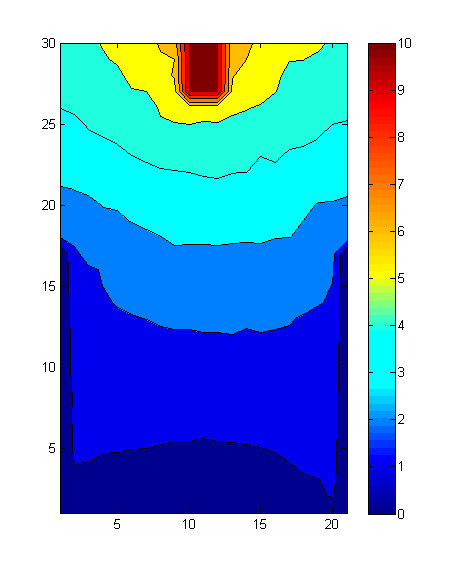
\includegraphics[scale=0.4]{duzycontourmap}
	\caption{Powierzchnie ekwipotencjalne dla kondensatora cylindrycznego, uzyskane w rozdzielczości 1 V}
\end{figure}

\begin{figure}[h!]
	\centering
	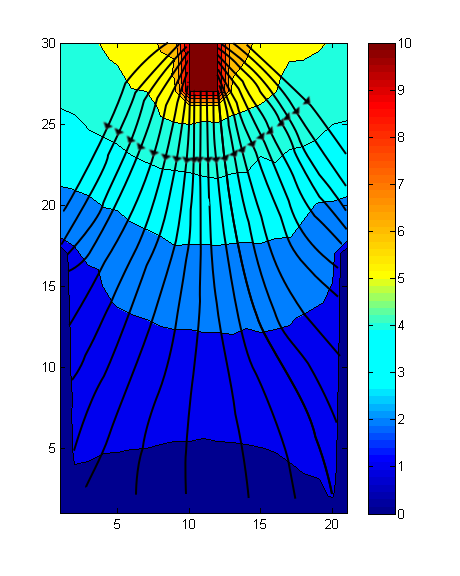
\includegraphics[scale=0.4]{duzycontourmapLINIE}
	\caption{Dorysowane "ręcznie" linie natężenia pola wewnątrz i na zewnątrz kondensatora}
\end{figure}
\clearpage
\subsubsection{Wyniki obliczeń natężenia pola w wybranych punktach dla dowolnego układu elektrod}

\begin{table}[h!tbp]
\centering
\begin{tabular}{|r|r|r|r|}
\hline
\multicolumn{1}{|l|}{Nr punktu} & \multicolumn{1}{l|}{$E_{x} [\frac{V}{m}]$} & \multicolumn{1}{l|}{$E_{y} [\frac{V}{m}]$} & \multicolumn{1}{l|}{$|E| [\frac{V}{m}]$} \\ \hline
1 & 1 & 16 & 16.03 \\ \hline
2 & 3 & 13 & 13.34 \\ \hline
3 & -8 & 5 & 9.43 \\ \hline
\end{tabular}
\label{}
\caption{Wyniki obliczeń natężenia pola elektrycznego w wybranych punktach}
\end{table}

%----------------------------------------------------------------------------------------
%	SECTION 6
%----------------------------------------------------------------------------------------
\section{Wnioski}

Dzięki doświadczeniu zapoznaliśmy się z metodami wyznaczania pola elektrycznego oraz modelami teoretycznymi dla różnych rodzajów kondensatorów. Poznaliśmy sposób obliczania natężenia pola na podstawie pomiarów potencjału elektrycznego, wykonywania ilustracji powierzchni ekwipotencjalnych oraz linii pola przy pomocy oprogramowania naukowego i grafiki wektorowej.
%----------------------------------------------------------------------------------------
%	BIBLIOGRAPHY
%----------------------------------------------------------------------------------------

\bibliographystyle{apalike}

\bibliography{sample}
%----------------------------------------------------------------------------------------


\end{document}
